%increment counter by one, such that advertisement lecture doesn't skew chapter numbering
\setcounter{chapter}{11}
\chapter{Lecture twelve: Connection of Components}
\section{Connecting components}
\subsection{Results}
A revised class diagram for the components of the system. An architecture includes dependencies between components. The implementation of these dependencies must be designed. The dependencies are designed as connections between the classes in the components. The revised class diagram specifies these connections precisely. 
\begin{figure}[H]
    \centering
    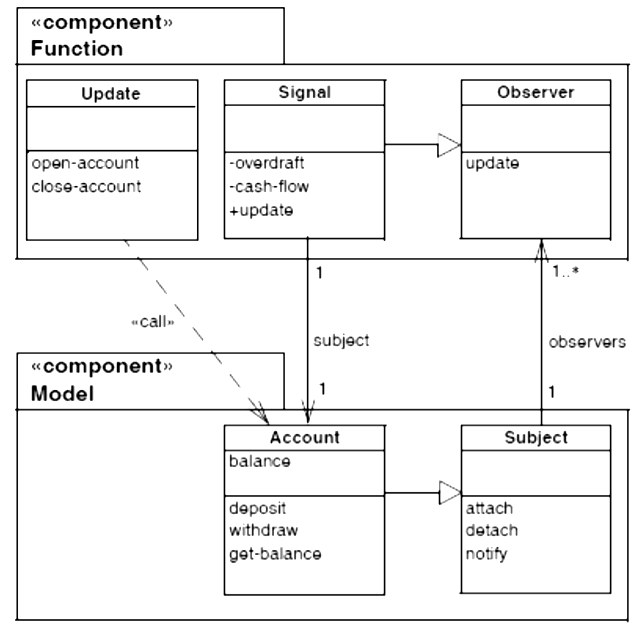
\includegraphics[width=0.5\textwidth]{figures/connectingcomponentsresult.png}
\end{figure}

\subsection{Activities}
From the class diagram and component specifications, you connect classes, and explore patterns, which leads to evaluating connections, which leads to a revised class diagram and component specifications.

\begin{figure}[H]
    \centering
    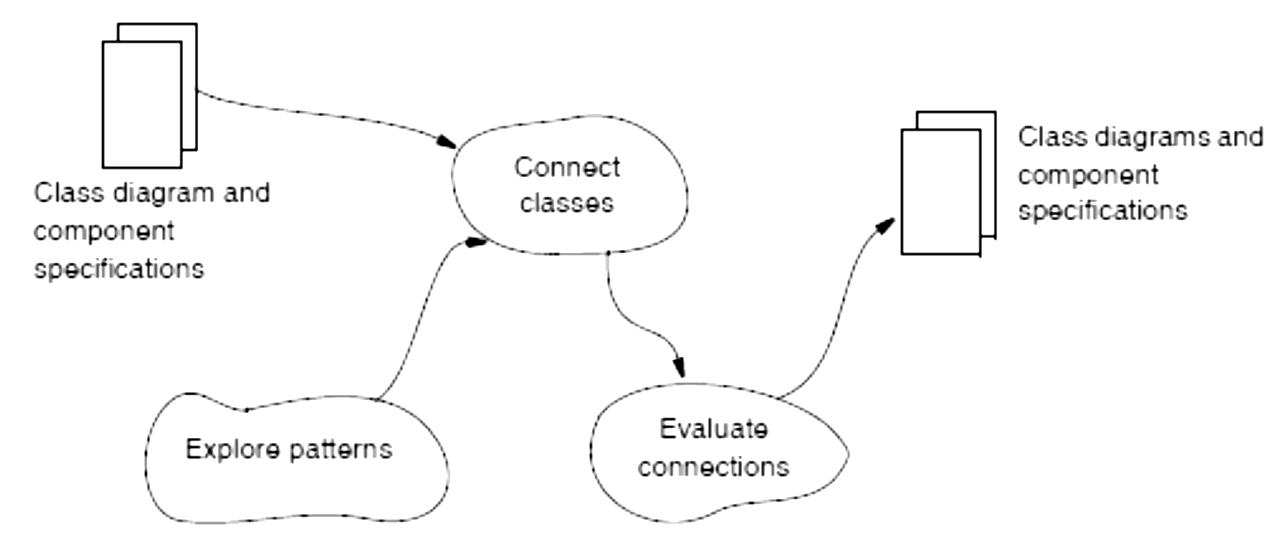
\includegraphics[width=0.5\textwidth]{figures/connectingcomponentsactivities.png}
\end{figure}

\subsection{Key concepts}

\section{Connect classes}
\begin{itemize}
    \item \textbf{Component:} A collection of program parts that constitutes a whole and has well-defined responsibilities.
    \item \textbf{Connection:} Realisation of a dependency between components.
\end{itemize}

These utilise \textbf{aggregation, specialisation, and calls}.

\begin{figure}[H]
    \centering
   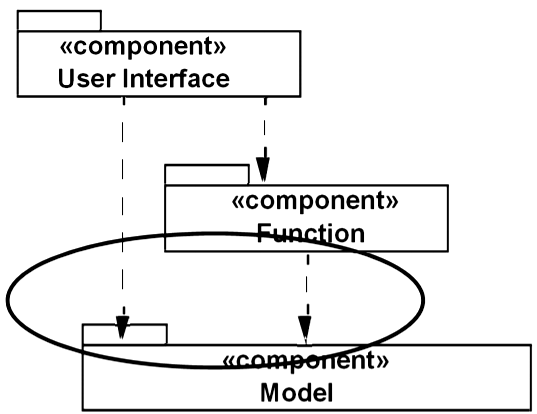
\includegraphics[width=0.4\textwidth]{figures/connectclasses.png}
\end{figure}

\section{Connection}
\subsection{Aggregation}

A dependency can be realised by letting a class in one component aggregate a public class from another component.

\begin{figure}[H]
    \centering
   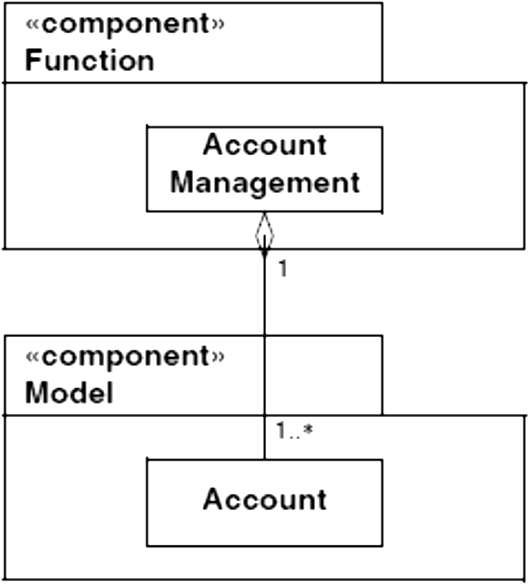
\includegraphics[width=0.3\textwidth]{figures/connectionaggregation.png}
\end{figure}

\subsection{Specialisation}

A dependency can be realised by defining a class in one component as a specialisation of a public class in another component.

\begin{figure}[H]
    \centering
   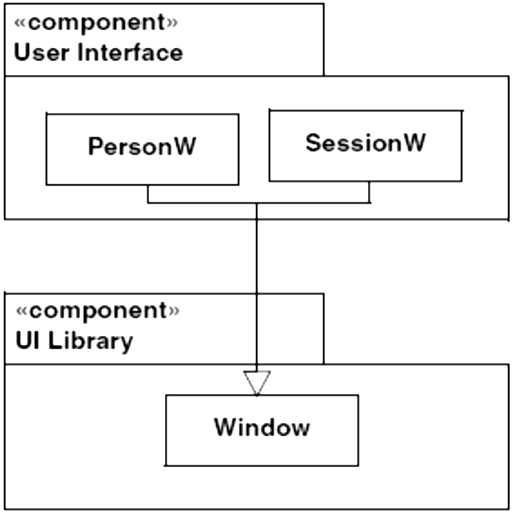
\includegraphics[width=0.3\textwidth]{figures/connectionspecialization.png}
\end{figure}

\subsection{Call}

A class in one component calls a public operation in another component.

\begin{figure}[H]
    \centering
   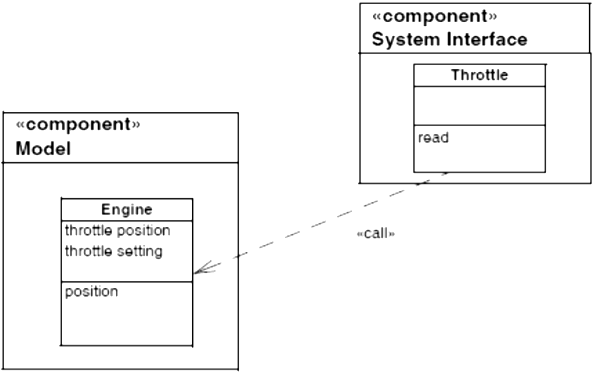
\includegraphics[width=0.5\textwidth]{figures/connectioncall.png}
\end{figure}

\section{Explore patterns}

There are patterns for realising dependencies between classes. The most general of these patterns is called \textbf{Observer pattern}. In this pattern the \textbf{Subject} knows its observers and provides for attaching and detaching observers. The \textbf{Observer} provides an update operation to the subject. The involved objects are all from either Concrete subject or Concrete observer. The \textbf{Concrete subject} notifies its observers when its state has changed. The \textbf{Concrete observer} each know their concrete subject and each implement the update operation.

\begin{figure}[H]
    \centering
   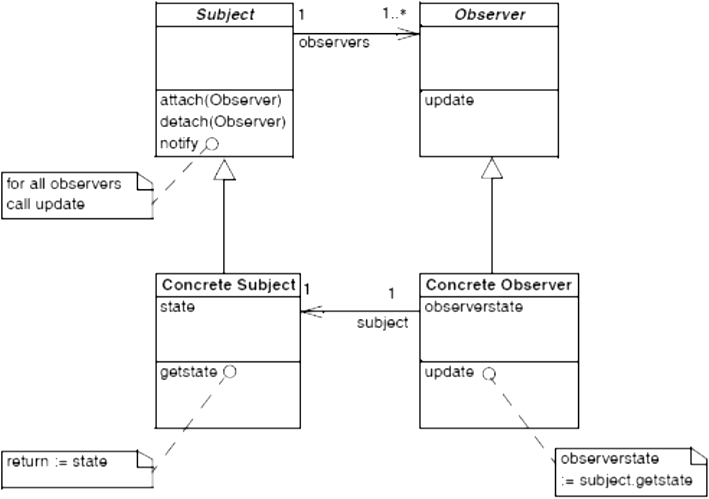
\includegraphics[width=0.65\textwidth]{figures/explorepatterns.png}
\end{figure}

\subsection{Using the observer pattern}

The account is the \textbf{Concrete subject}. The signal class contains the operations to observe the state of an Account object.

\begin{figure}[H]
    \centering
   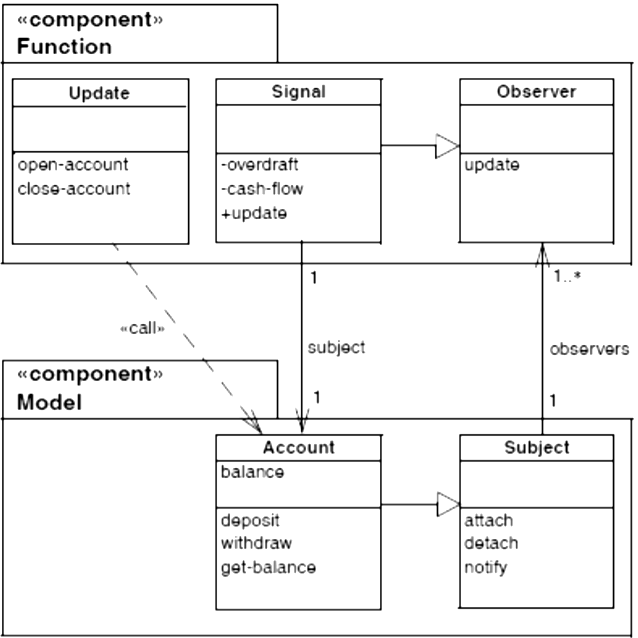
\includegraphics[width=0.4\textwidth]{figures/observerpattern.png}
\end{figure}


\section{Evaluate connections: Coupling and Cohesion}
\textbf{Coupling} is the degree to which a class or component knows about another class or components. \textbf{Loose coupling} is all interaction that goes through the interface. \textbf{Cohesion} is the degree to which a class or component has a single, well-focused purpose. \textbf{High cohesion} is a clear purpose. 
Coupling and cohesion are structural measures that we asses by evaluating the class diagrams for the involved components. The two measures points in opposite directions. If a cohesive class is split, the resulting classes will be tightly coupled. If two classes with low coupling are integrated, the resulting class will be incohesive. 
\begin{figure}[H]
    \centering
   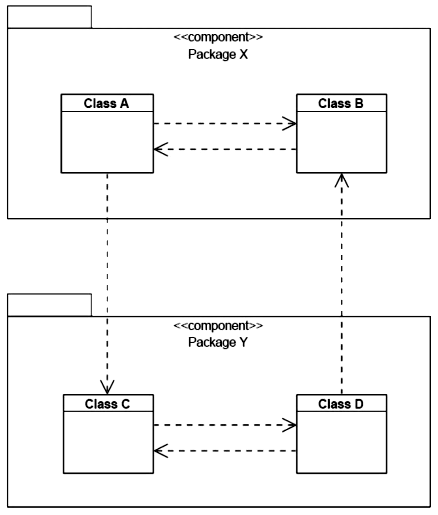
\includegraphics[width=0.3\textwidth]{figures/evaluateconnectionsboth.png}
\end{figure}

\subsection{Coupling}
\textbf{Coupling:} A measure of how closely two classes or components are connected. \\
Coupling expresses that change in one class or component necessitates change in another class or component. The ideal state is \textbf{low coupling}. Two classes or components have high coupling if changes in one requires changes in the other. Coupling is a negative property, and should be minimised. In increasing order of coupling;

\begin{itemize}
    \item Outside coupling; refer directly to public operations in another class or component
    \item Inside coupling; refer directly to private properties in the same class or component
    \item Coupling from below; refer from a specialisation to a private property in the generalisation
    \item Sideways coupling; refer directly to private properties in another class or component
\end{itemize}

Obtain low coupling by using outside coupling, and avoid sideways. Achieving this is not difficult in OOP, as classes makes encapsulation possible.

\begin{figure}[H]
    \centering
   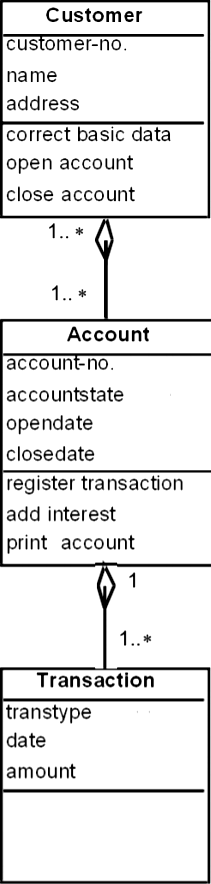
\includegraphics[width=0.15\textwidth]{figures/cohesion.png}
\end{figure}

\subsection{Cohesion}
\textbf{Cohesion:} A measure of how well a class or component is tied together. \\
Cohesion expresses that a class or component constitutes a whole with essential relations between its parts. If cohesive classes/components are split, high degree of coupling will follow. Cohesion is positive, that should be pursued. Cohesion leads to greater comprehensibility, cohesive programs contain fewer errors and costs less to develop and maintain. This leads to higher quality programs.
The ideal state is \textbf{high cohesion}. 

When looking at \textbf{classes} and \textbf{objects} The following properties correlate with high cohesion:
\begin{itemize}
    \item Operations constitute a functional whole
    \item Attributes and object structures describe objects with well-defined states. 
    %\item The parts are conceptually related
    %\item The parts are functionally wholes
    %\item The parts reflect well-defined states
    \item Operations use each other
\end{itemize}

When looking at component cohesion, the following features point to cohesive components:
\begin{itemize}
    \item Component classes are conceptually related
    \item Structural relations among classes are primarily generalisations and aggregations
    \item Key operations can be carried out within the component
\end{itemize}

\subsection{Evaluate connections}

\begin{figure}[H]
    \centering
    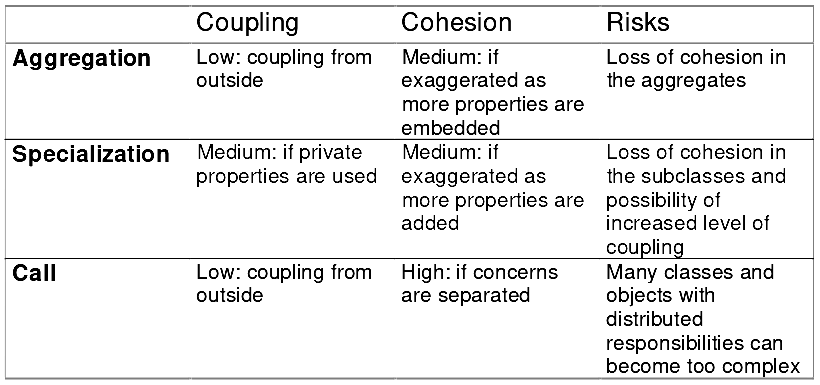
\includegraphics[width=0.5\textwidth]{figures/evaluateconnections.png}
\end{figure}

\section{Summary}

\begin{figure}[H]
    \centering
    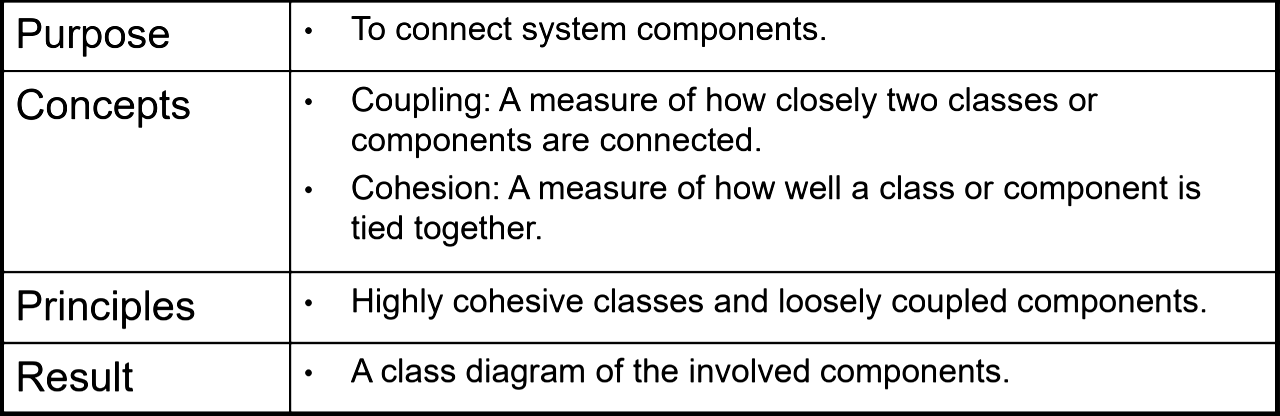
\includegraphics[width=0.7\textwidth]{figures/connectingcomponentssummary.png}
\end{figure}